después de haber definido qué es $\ln(x)$ podemos extender $\log_e(x)$ para significar $\ln(x)$.

Por supuesto, después de haber definido y demostrado todo rigurosamente podemos escribir las cosas en cualquier orden, pero esto solo debe hacerse una vez el estudiante ha obtenido un entendimiento sólido sobre por qué estas retrocompatibilidades funcionan.

En una nota menos técnica desearíamos señalar que elegir $e^x$ para representar fenómenos exponenciales en disciplinas como la física o la estadística es meramente una decisión estética. Uno podría perfectamente expresar $2^3$ como $\pi^{\log_{\pi}(2)\cdot 3}$, es solo que al elegir $e^x$, solo las constantes relevantes --- las que de verdad poseen significado semántico en el universo --- permanecen.

\newpage

Véase el caso del decaimiento exponencial. Si se tiene un material radioactivo, se puede medir cuántos isótopos radioactivos tiene ($N_0$). Con el paso del tiempo ($t$), algunos de esos isótopos se desintegrarán, transformándose en otros elementos o isótopos y dejando una menor cantidad de isótopos radioactivos en el material ($N(t)$). Este proceso también es una exponencial, y por ende puede expresarse con la siguiente ecuación diferencial:

$$N'(t) = -\lambda N(t)$$

Una posbile solución a esta ecuación es

$$N(t) = N_0 a^{-ct}$$

Donde $c = \lambda \cdot \log_a(e)$. Esto es, sin falta, una solución válida. Su único problema, como hemos dicho, es uno estético. ¿Qué significa $c$? ¿Podría uno saber algo acerca del fenómeno descrito solo mirando a esta constante? De ninguna manera. Si en su lugar lo expresamos así:

$$N(t) = N_0 e^{-\lambda t}$$

De repente no hay \enquote{constantes basura} y, más importantemente, $\lambda$ adquiere significado semántico. En el caso de la desintegración radioactiva, $\lambda$ es llamada la \textit{constante de desintegración} o \textit{decaimiento}. Esto no solo es relevante para $\lambda$, sino para todas las magnitudes que se deriven de ella. Por ejemplo, $t_{1/2} = \frac{\ln(2)}{\lambda}$ es la \textit{semivida} de la cantidad, y describe la cantidad de tiempo necesaria para que la cantidad $N$ se reduzca a la mitad. ¿Podríamos haber expresado lo mismo arrastrando un factor de $\log_a(e)$ constantemente? Totalmente, pero entonces nuestra definición de semivida sería algo como \enquote{la cantidad de tiempo necesaria para que la cantidad $N$ se reduzca a la mitad dividida por $\log_a(e)$}. Esta definición simplemente se siente embrollada y mal, mientras que la otra parece arrastrar cierto significado objetivo, como si la constante $e$ fuese la elección \textit{natural} de base. Esto es lo que hace \textit{natural} al logaritmo natural.

En resumen, las variables exponenciales son aquéllas cuya tasa de cambio es proporcional al valor de la variable en sí, y $e$ es el número que cumple que esa constante de proporcionalidad es $1$, lo que lo hace la forma más \textit{natural} de expresar muchas ecuaciones en física.

\subsection{Números complejos como rotaciones.}

Cuando se presentan los números complejos por primera vez, una de las extrañas decisiones que destacan sobre su definición es su posición en el plano complejo. Aunque cualquier par ordenado puede ser ubicado en una gráfica, no es evidente por qué $i$ debería estar a un paso del $0$ perpendicular al eje real. Sin embargo, cuando movemos nuestra perspectiva sobre los números para pensar en ellos como \textit{acciones}, esto no solo se convierte en un resultado razonable, sino en el único posible.

Si uno está familiarizado con simples vectores en $\mathbb{R}^2$, uno ya vislumbrará cómo los números pueden ser vistos de esta manera. Multiplicar un vector por un número positivo es \textit{escalarlo}, hacerlo más grande o más pequeño preservando la dirección a la que \enquote{apunta}. De manera similar, multiplicarlo por un número negativo corresponde a hacer lo mismo pero \enquote{volteando} su dirección, o rotándolo por $180^{\circ}$.

¿Pero qué es una rotación de $180^{\circ}$ si no dos rotaciones consecutivas de $90^{\circ}$? Si multiplicar por $-1$ produce una rotación de $180^{\circ}$, aquél número que represente una rotación de $90^{\circ}$ ha de ser, en cierto sentido, la raíz cuadrada de $-1$. Esta noción de multiplicaciones (de números) transformándose en sumas (de ángulos) debería dar una pista de que las exponenciales entrarán en escena tarde o temprano.

Si uno no queda convencido con este argumento, nótese lo siguiente. Si $z = a + bi$, entonces $i\cdot z = -b + ai$. Esta transformación de coordenadas es exactamente lo mismo que una rotación antihoraria de $90^{\circ}$ ($(x, y) \to (-y, x)$). Este concepto puede extrapolarse a otros números complejos, sin embargo nuestro caso solo requiere que entendamos la acción de $i$.

\subsection{Exponenciales complejas.}

Esta es quizás la parte más difícil de visualizar, así que usaremos una analogía con la física. Puede ser útil interpretar $f(t) = \exp(it)$ como la posición de una partícula en el plano complejo en cierto punto en el tiempo, y su derivada $f'(t) = i\exp(it)$ como su velocidad. Vale la pena notar que, en cualquier posición, el vector velocidad de la partícula forma un ángulo de $90^{\circ}$ con su vector posición (pues $f'(t) = i\cdot f(t)$, esto es, una rotación antihoraria de $90^{\circ}$. Uno puede visualizar a la partícula \enquote{orbitando} en torno al origen en un movimiento circular (Figura \ref{rot}).

\begin{figure}[H]
	\centering
	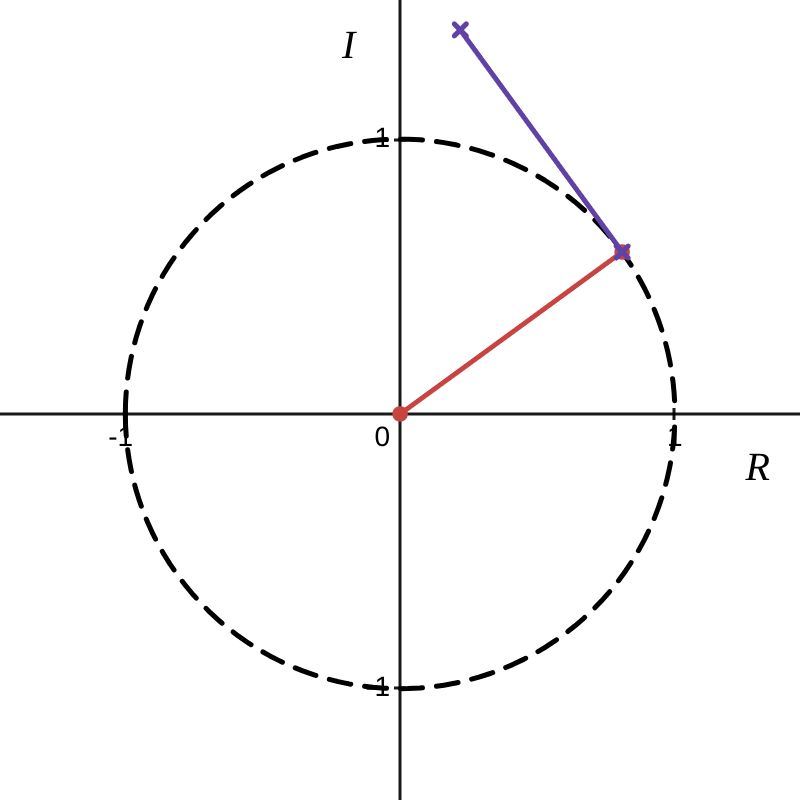
\includegraphics[width=\linewidth]{media/rotation.png}
	\caption{Partícula en el plano complejo con posición $\exp(it)$ (señalada en rojo) y velocidad $i\exp(it)$ (señalada en morado). Al principio, $f(0) = 1$. Después de un cambio infinitesimal en el tiempo, la partícula se habrá movido perpendicular a su vector posición (a lo largo de su vector velocidad). Como sabemos por la física, este es el escenario para el movimiento circular. Un gráfico interactivo de Desmos está disponible en \url{https://www.desmos.com/calculator/8npnlxgjba}.}
	\label{rot}
\end{figure}

Lo que nos dice la fórmula de Euler es que el ángulo barrido por el vector posición de la partícula en un tiempo $t$ es \textit{exactamente} $t$. Entonces, tras 2 segundos, la partícula forma un ángulo de 2 radianes con el eje real; después de $\pi$ segundos, la partícula forma un ángulo de $\pi$ radianes con el eje real (lo cual coincide con el punto $-1 + 0i$), etc.

Nuevamente, la función exponencial aquí no es una decisión fundamental. Podríamos perfectamente haber elegido el número áureo $\phi$ como una base, haciendo que $f(t) = \phi^{it}$. La única diferencia es que en este caso, los ángulos barridos no coinciden con el tiempo transcurrido. Usando esta función, llegamos a la fórmula de EulErik (nombrada así por ningún motivo en particular):

$$\phi^{i\frac{\pi}{\log_{\phi}(e)}} = -1$$

\section{Conclusión.}

Para condensar todo lo visto hasta ahora en un resumen sencillo:

\begin{itemize}
	\item Los números complejos proporcionan una forma de expresar rotaciones en el plano complejo. Concretamente, $i$ significa una rotación antihoraria de $90^{\circ}$.
	\item La función exponencial ($\exp(x)$ o $e^x$) proporciona una forma de expresar variables cuya tasa de cambio es igual a su valor actual. Su característica más fundamental es el hecho de que su derivada es igual a sí misma.
	\item $e^{it}$ es el punto que resulta de rotar un punto en torno al origen por tiempo $t$, y por propiedades expuestas de $\exp(x)$, este caso particular satisface que el tiempo transcurrido es igual al ángulo barrido por el vector posición del punto. Otra forma de expresar la posición de este vector es $\cos(x) + i\sin(x)$ (la fórmula de Euler).
	\item $e^{i\pi}$ es el caso particular donde el punto aterriza en $-1$ (la identidad de Euler).
\end{itemize}
